\documentclass[12pt,a4paper]{report}
\usepackage[brazil]{babel}
\usepackage[]{algorithm}
\usepackage[]{algorithmic}
\usepackage[style=numeric,backend=biber]{biblatex}
\usepackage[utf8]{inputenc}
\usepackage{kpfonts}
\usepackage[T1]{fontenc}
\usepackage{wrapfig}
\usepackage{graphicx}
\usepackage{enumerate}
\usepackage{subcaption}
\usepackage{float}
\usepackage{caption}
\usepackage{listings}
\usepackage{lipsum}
\usepackage{amsthm}
\usepackage{amssymb}
\usepackage{bm}
\usepackage{color}
\usepackage{afterpage}
\usepackage[inline]{enumitem}
\usepackage{pdflscape}
\usepackage{listingsutf8}
\usepackage{siunitx}
\usepackage{bashful}

\graphicspath{ {./images/} }

\lstset{frame=tb,
  aboveskip=2mm,
  belowskip=2mm,
  showstringspaces=false,
  columns=flexible,
  basicstyle=\footnotesize,,
  numbers=left,
  numbersep=5pt,
  stepnumber=1,
  breaklines=true,
  keepspaces=true,
  breakatwhitespace=true,
  showtabs=false,  
  tabsize=2
}

% Definindo estilo para os códigos
\definecolor{mGreen}{rgb}{0,0.6,0}
\definecolor{mGray}{rgb}{0.5,0.5,0.5}
\definecolor{mPurple}{rgb}{0.58,0,0.82}
\definecolor{dkgreen}{rgb}{0,0.6,0}
\definecolor{backgroundColour}{rgb}{0.97,0.97,0.97}

\lstset{basicstyle=\ttfamily,
    backgroundcolor=\color{backgroundColour},   
    commentstyle=\color{mGreen},
    keywordstyle=\color{magenta},
    numberstyle=\tiny\color{mGray},
    commentstyle=\color{dkgreen},
    stringstyle=\color{mPurple},
    basicstyle=\footnotesize,
    breakatwhitespace=false\textbf{,}         
    breaklines=true,                 
    captionpos=b,                    
    keepspaces=true,                 
    numbers=left,                    
    numbersep=5pt,                  
    showspaces=false,                
    showstringspaces=false,
    showtabs=false,                  
    tabsize=2,
    language=bash
}

\lstdefinestyle{BStyle}{
    backgroundcolor=\color{backgroundColour},  
    showstringspaces=false,
    numbers=none,
    language=bash
}

\pagenumbering{arabic}
\renewcommand{\thesection}{\arabic{section}}

\bibliography{ref}
\renewcommand{\contentsname}{Sumário}{\thispagestyle{empty}}
\renewcommand{\baselinestretch}{1.5} 

\begin{document}

\begin{titlepage}
    \begin{center}
        \vspace*{1cm}
        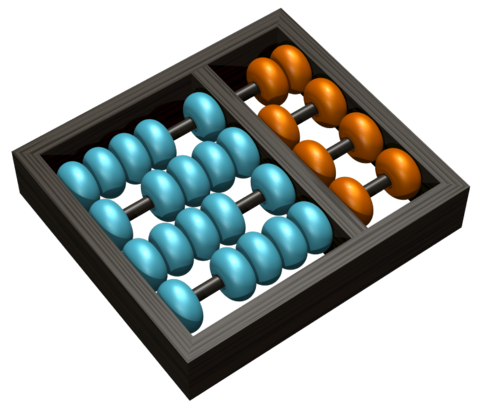
\includegraphics[width=0.25\textwidth]{Logo}\\
        \vspace{1.5cm}
        \Huge
    	\textbf{MC833 Relatório 4 \\
        Backlog e Processos Zumbis} \\
        \vspace{1.5cm}
        \Large
        \textbf{Aluno}: Fábio Camargo Ricci\\
        \textbf{RA}: 170781\\
        \vspace{1.2cm}
    	\Large 
    	Instituto de Computação\\
    	Universidade Estadual de Campinas\\
    	\vspace{1.5cm}
        Campinas, 24 de Outubro de 2021.
    \end{center}
\end{titlepage}
\tableofcontents
\clearpage

\newcommand{\shellcmd}[1]{\texttt{\footnotesize\# #1}}%estilizando citação de comandos do shell

\section{Questões}

\begin{enumerate}
    \item Com o conhecimento adquirido em aula explique qual a relação entre \textbf{backlog} e número de conexões.
    
    \item Descreva o processo de troca de pacotes durante o estabelecimento da conexão com as filas mantidas pelo TCP para um socket de escuta.
    
    \item Descreva como é a implementação do \textbf{backlog} de um socket TCP no kernel linux (para versão 2.2 ou mais recentes), e em seguida indique o valor padrão do backlog. (Inclua figuras no seu relatório verificando esse valor padrão do backlog). Qual a diferença entre os valores de \textbf{net.ipv4.tcp\_max\_syn\_backlog} e \textbf{net.core.somaxconn}?
    
    \item Modifique o código do servidor do exercício anterior de modo que o valor do backlog passado para a função listen seja um argumento na linha de comando. Realize experimentos a fim de verificar quantos clientes conseguem de imediato conectar-se ao servidor (conexões em estado ESTABLISHED) para valores de backlog desde 0 até 10. Elabore um esquema para tentar conectar 10 clientes de forma simultânea. Os resultados obtidos condizem com o esperado?
    
    \item É correto afirmar que o código na versão atual gera processo zumbi? Explique. Se a sua resposta foi sim, então altere o código da questão 4 de modo que os processos criados pelo fork sejam corretamente finalizados ao invés de permanecerem no estado zumbi quando um cliente encerra sua conexão. Indique as mudanças feitas no código.
\end{enumerate}

\section{Respostas}

\begin{enumerate}
    \item Em teoria, o backlog se refere ao número de conexões ativas (estabelecidas) mais o número de conexões pendentes. Dessa forma, o servidor é limitado a ter um número de conexões concorrentes quanto o backlog permitir, ignorando mensagens SYN quando fila está cheia.
    \\
    Apesar disso, cada sistema operacional pode implementar o controle do backlog (ao chamar o método \textbf{listen}) de uma maneira, de modo que o tamanho real das filas nem sempre segue essa lógica estritamente.
    
    \item Quando um cliente deseja iniciar uma conexão, envia um pacote com a flag \textbf{SYN} ativada, especificando o número da porta desejada. O servidor por sua vez, coloca a conexão em um fila de conexões incompletas e responde um pacote com as flags \textbf{ACK} e a \textbf{SYN}. O cliente, por fim, envia um pacote com a flag \textbf{ACK}, completando assim o 3 way handshake. Com isso, o servidor move a conexão para a fila de conexões completas e o método \textbf{accept} pode retornar.
     
    \item Antes da versão 2.2 do linux, o backlog de um socket TCP determinava o número máximo de conexões aguardando um sinal \textbf{SYN} (conexões incompletas pendentes). Em versões futuras, o comportamento do backlog foi alterado, determinando o tamanho da fila de conexões no estado \textbf{ESTABLISHED}, as quais ja passaram pelo o handshake inicial do TCP (\textbf{SYN} e \textbf{SYN ACK}) e estão esperando por um \textbf{accept}.
    \\
    Dessa forma, o linux possui dois tamanhos de fila, uma para conexões aguardando \textbf{SYN} e outra para aquelas aguardando \textbf{accept}. Caso a primeira esteja cheia, o kernel irá ignorar novas conexões que chegam. Caso a segunda chegue no limite, todos os pacotes recebidos da conexão que causou overflow serão ignorados.
    \\ 
    O tamanho máximo da fila de conexões aguardando \textbf{SYN} é dado pelo parâmetro \textbf{tcp\_max\_syn\_backlog} (valor padrão 128). Já o tamanho da fila de \textbf{accept} é dado pelo backlog (passado como parâmetro na função \textbf{accept}), cujo valor máximo é dado pela constante \textbf{somaxconn} (valor padrão 128). Valores de backlog maiores que esse serão automaticamente truncados.
    \\
    Olhando o manual do linux, podemos observar:\\
    tcp\_max\_syn\_backlog:\\\\
    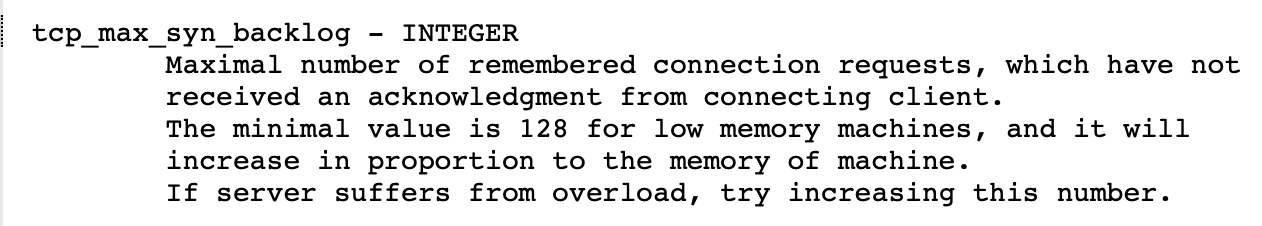
\includegraphics[width=1\textwidth]{images/tcp_max_syn_backlog.png}\\
    somaxconn:\\\\
    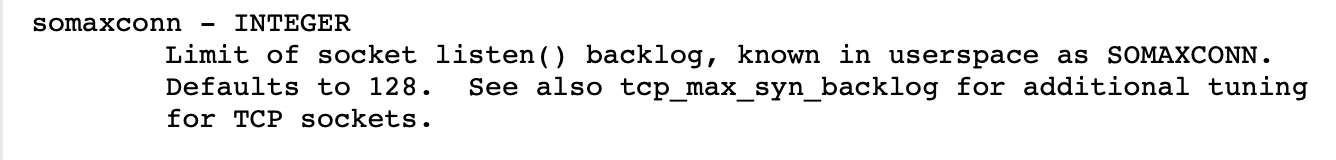
\includegraphics[width=1\textwidth]{images/somaxconn.png}
    
    \item Criou-se dois scripts para testar a conexão de clientes simultâneos, um que compila e executa o servidor (exec-server.sh - recebe como parâmetro o número de backlog) e um que compila e executa 10 clientes em paralelo (exec-clientes.sh - recebe como parâmetro o endereço IP e porta que o servidor está escutando). Repetiu-se o teste 10 vezes para números de backlog entre 1 e 10,  utilizando-se o comando \textit{lsof -iTCP:PORT} para realizar o monitoramento (Introduziu-se um \textbf{sleep(10)} para haver um janela de monitoramento das conexões). A seguir estão os resultados:
    \begin{enumerate} 
        \item Backlog = 1\\
        Servidor:\\\\
        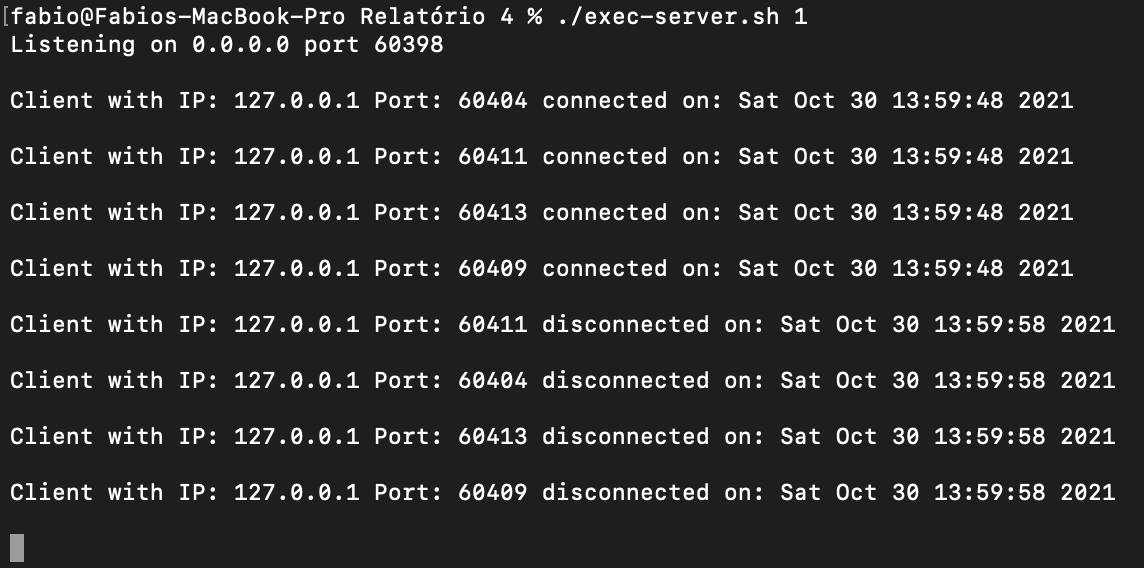
\includegraphics[width=1\textwidth]{images/servidor-backlog-1.png}
        Cliente:\\\\
        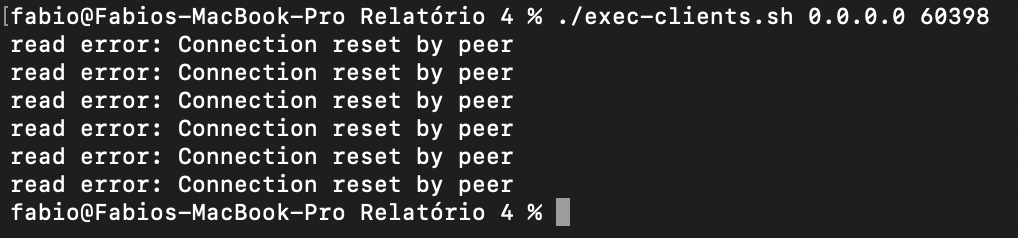
\includegraphics[width=1\textwidth]{images/cliente-backlog-1.png}
        Monitoramento:\\\\
        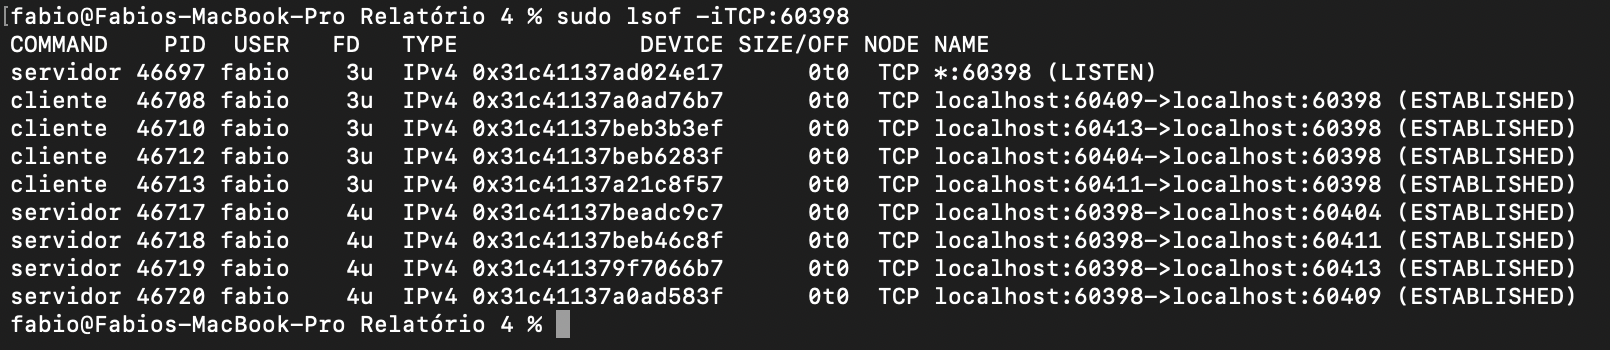
\includegraphics[width=1\textwidth]{images/lsof-backlog-1.png}
        
        \item Backlog = 2\\
        Servidor:\\\\
        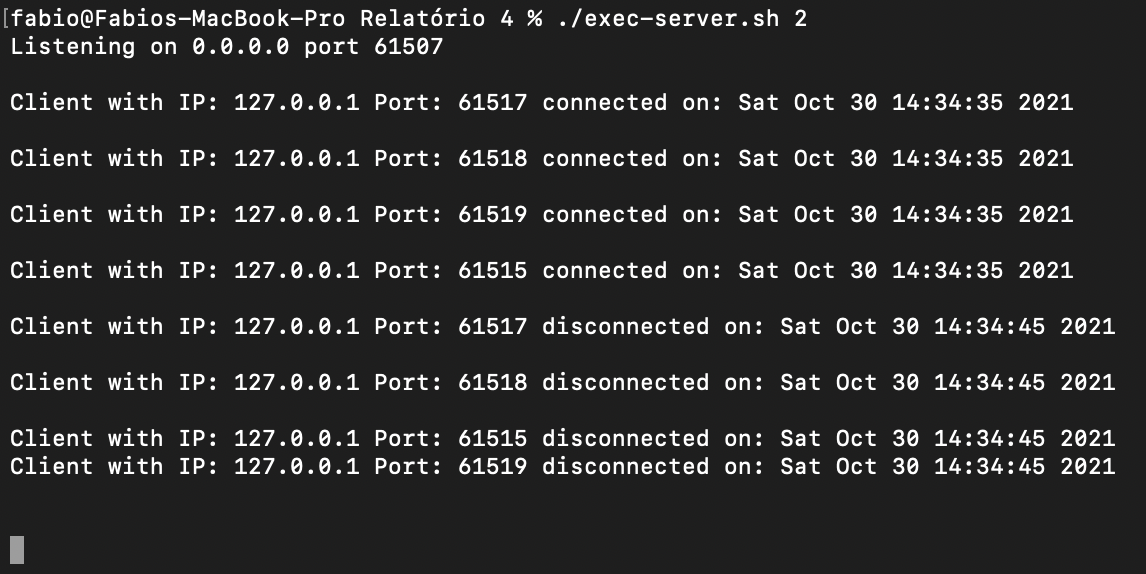
\includegraphics[width=1\textwidth]{images/servidor-backlog-2.png}
        Cliente:\\\\
        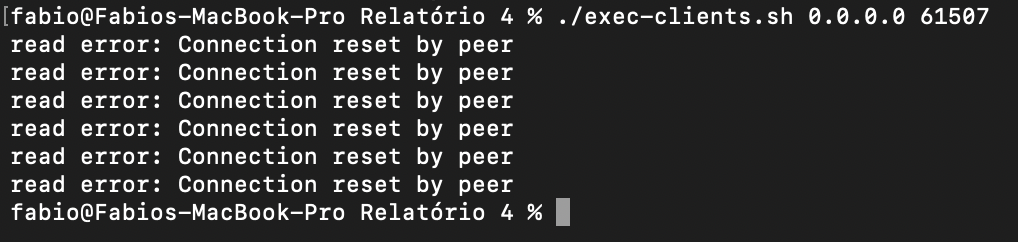
\includegraphics[width=1\textwidth]{images/cliente-backlog-2.png}
        Monitoramento:\\\\
        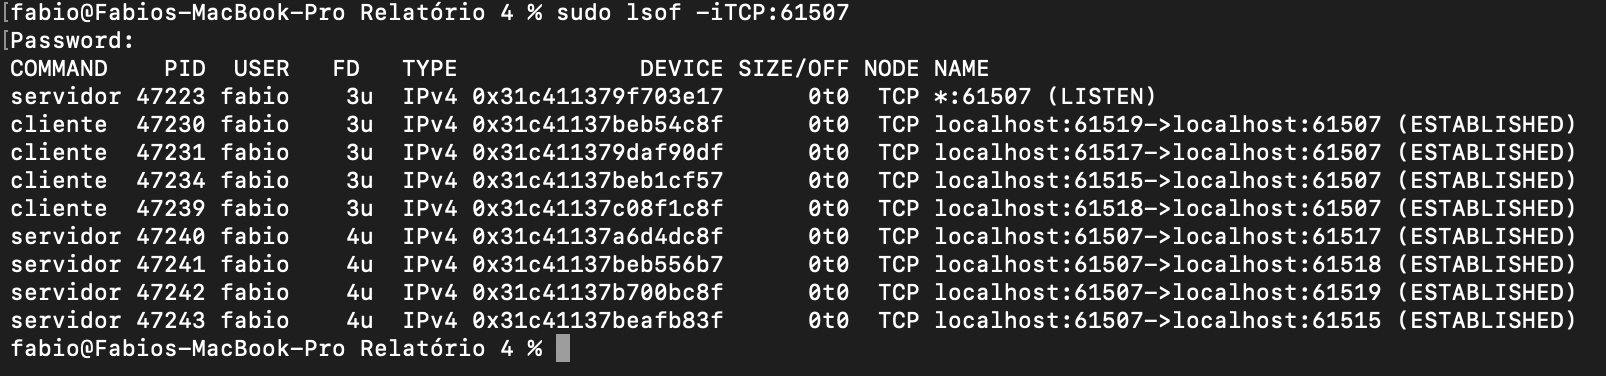
\includegraphics[width=1\textwidth]{images/lsof-backlog-2.png}
        
        \item Backlog = 3\\
        Servidor:\\\\
        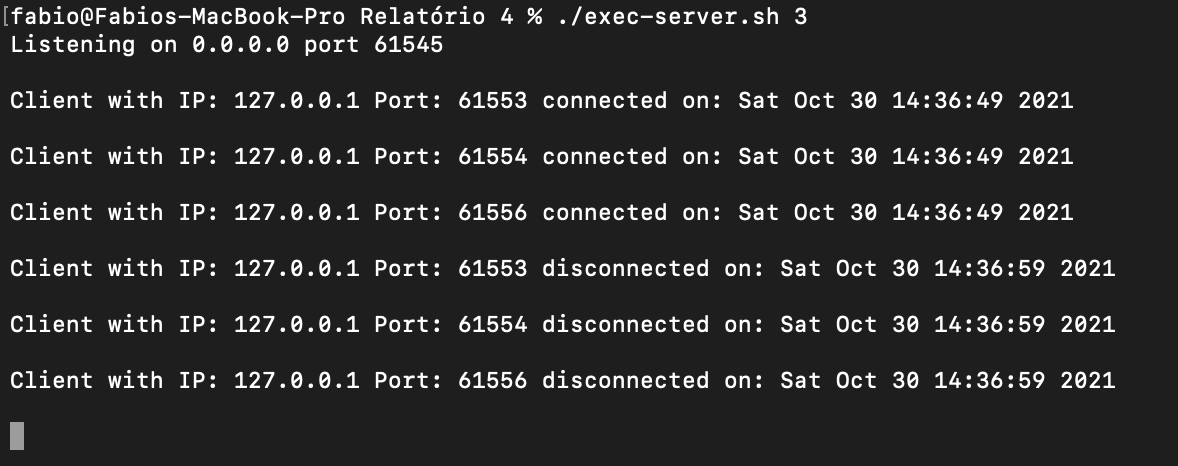
\includegraphics[width=1\textwidth]{images/servidor-backlog-3.png}
        Cliente:\\\\
        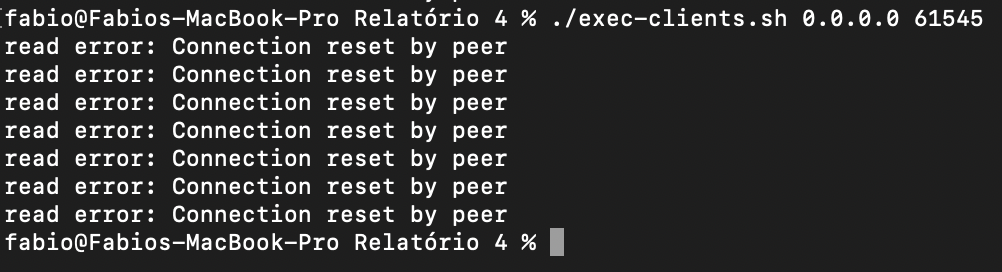
\includegraphics[width=1\textwidth]{images/cliente-backlog-3.png}
        Monitoramento:\\\\
        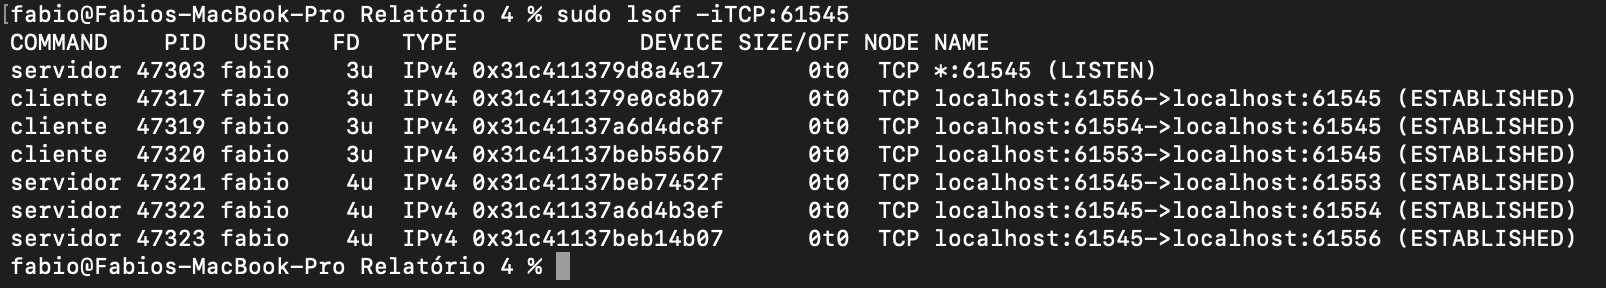
\includegraphics[width=1\textwidth]{images/lsof-backlog-3.png}
        
        \item Backlog = 4\\
        Servidor:\\\\
        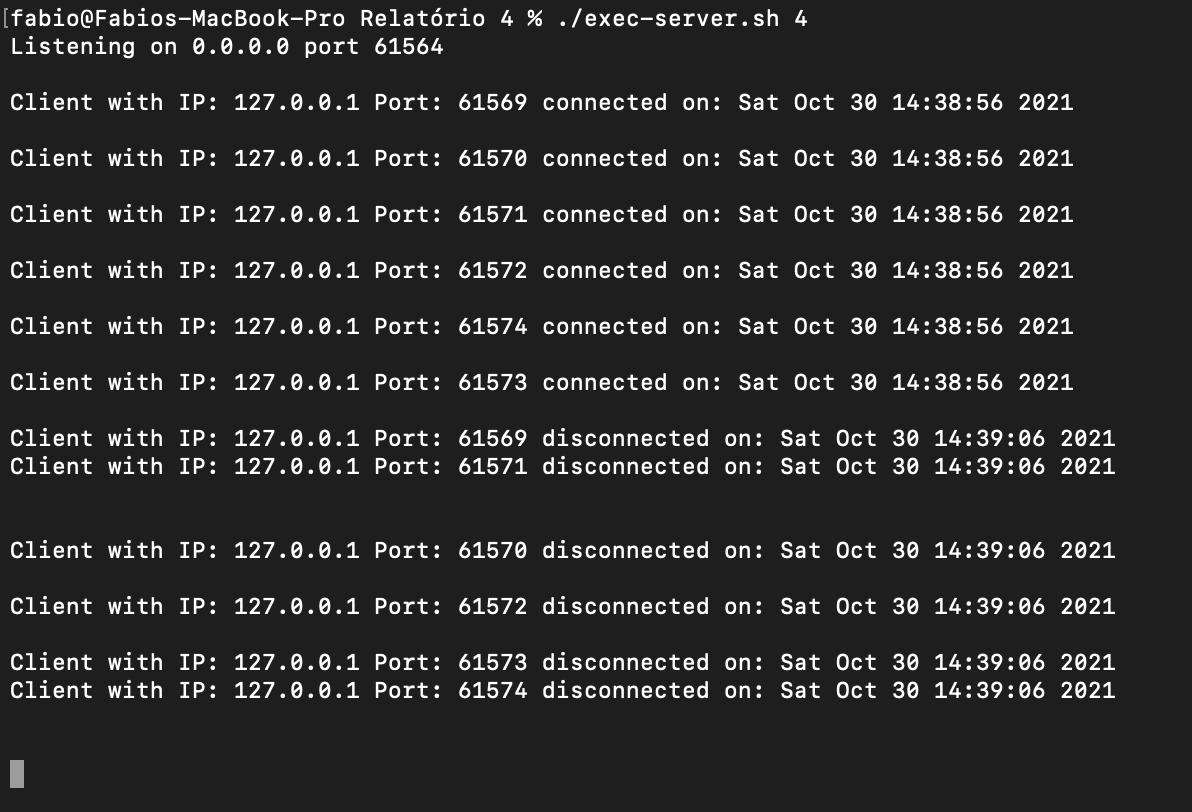
\includegraphics[width=1\textwidth]{images/servidor-backlog-4.png}
        Cliente:\\\\
        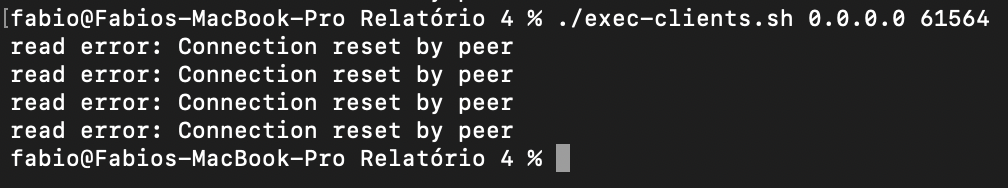
\includegraphics[width=1\textwidth]{images/cliente-backlog-4.png}
        Monitoramento:\\\\
        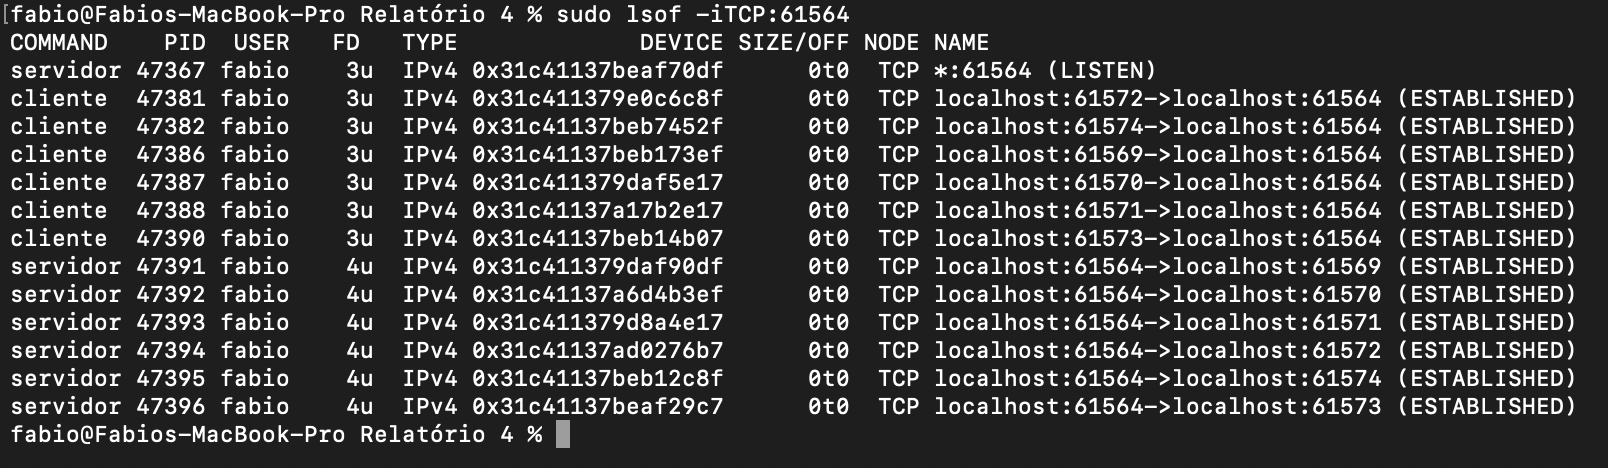
\includegraphics[width=1\textwidth]{images/lsof-backlog-4.png}
        
        \item Backlog = 5\\
        Servidor:\\\\
        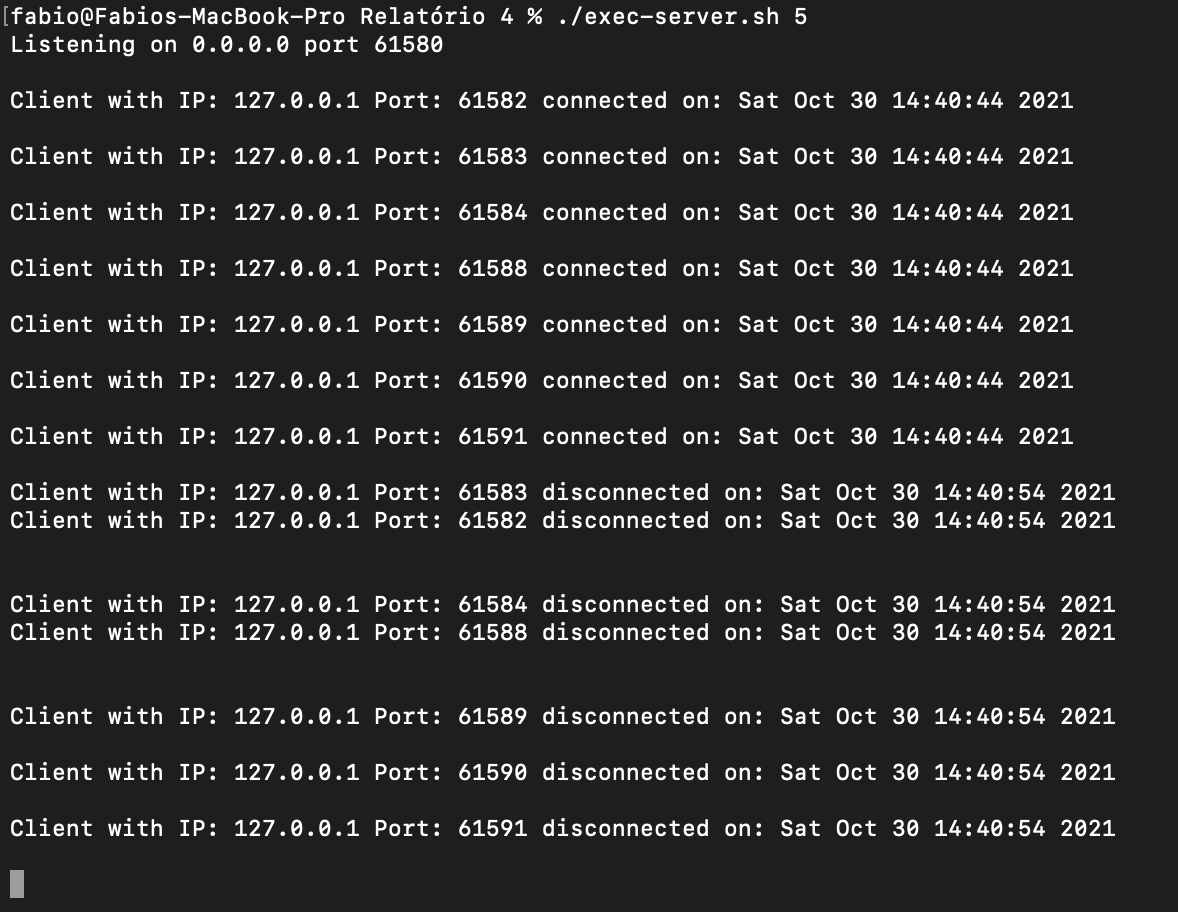
\includegraphics[width=1\textwidth]{images/servidor-backlog-5.png}
        Cliente:\\\\
        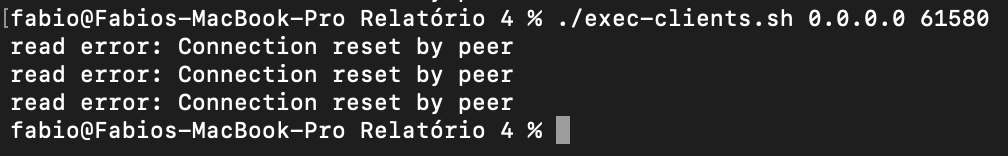
\includegraphics[width=1\textwidth]{images/cliente-backlog-5.png}
        Monitoramento:\\\\
        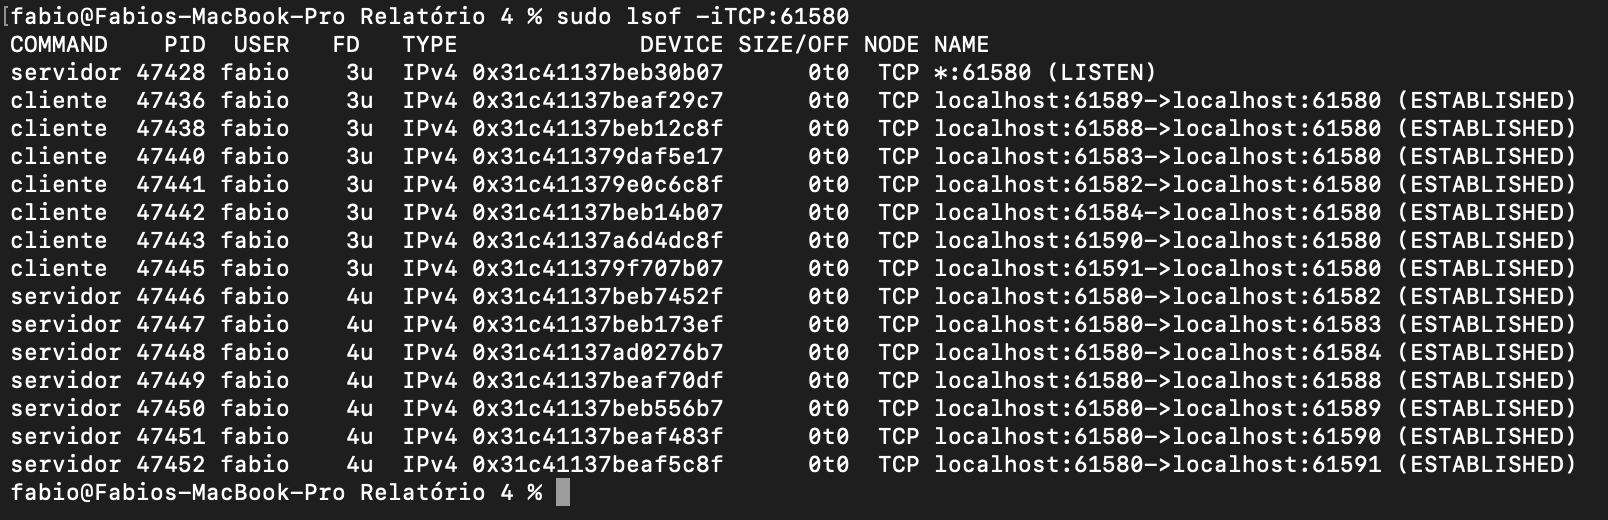
\includegraphics[width=1\textwidth]{images/lsof-backlog-5.png}
        
        \item Backlog = 6\\
        Servidor:\\\\
        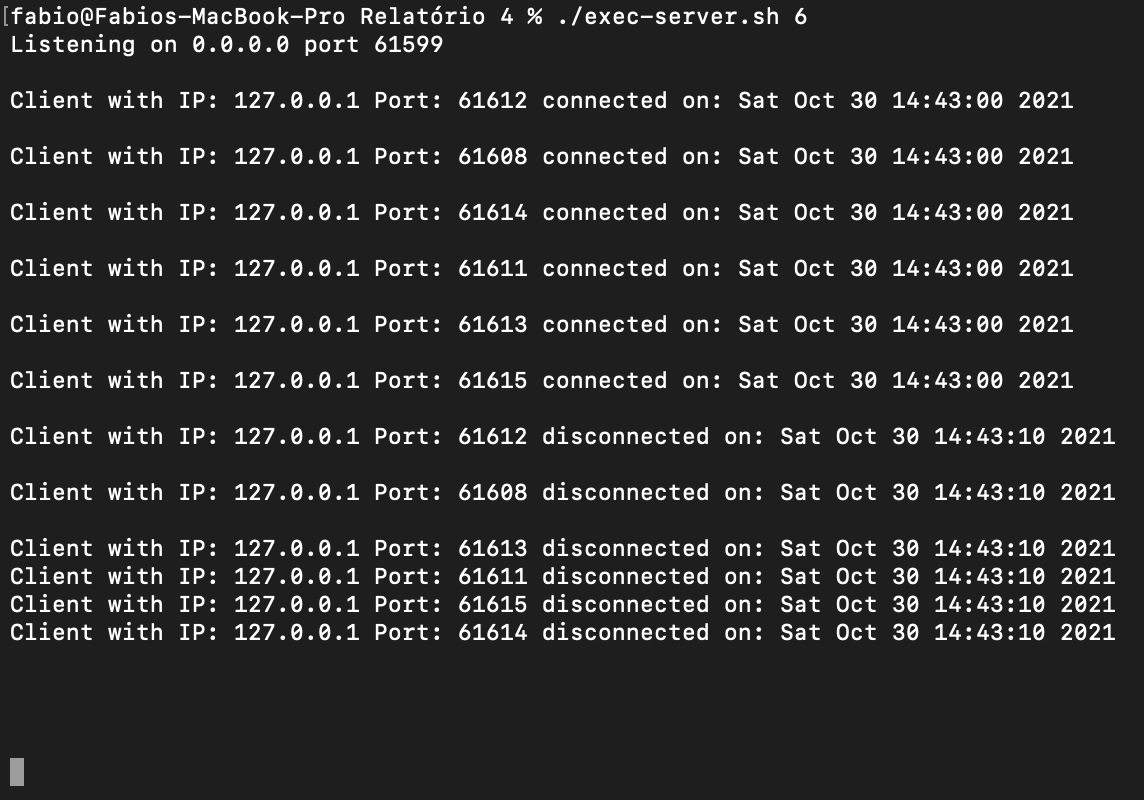
\includegraphics[width=1\textwidth]{images/servidor-backlog-6.png}
        Cliente:\\\\
        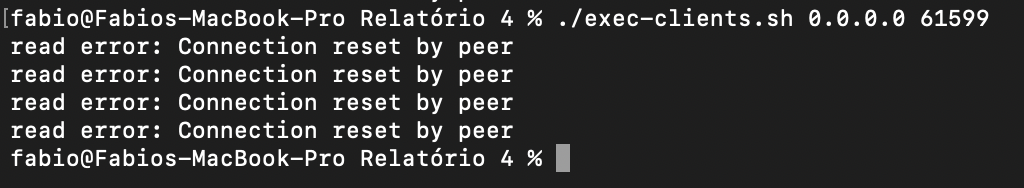
\includegraphics[width=1\textwidth]{images/cliente-backlog-6.png}
        Monitoramento:\\\\
        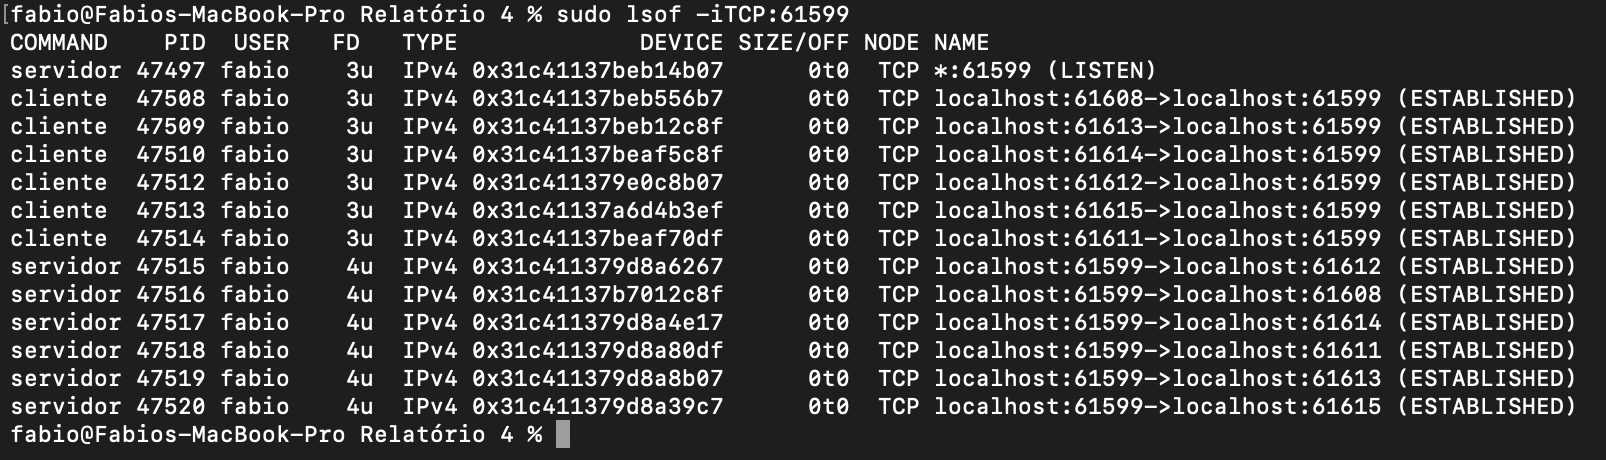
\includegraphics[width=1\textwidth]{images/lsof-backlog-6.png}
        
        \item Backlog = 7\\
        Servidor:\\\\
        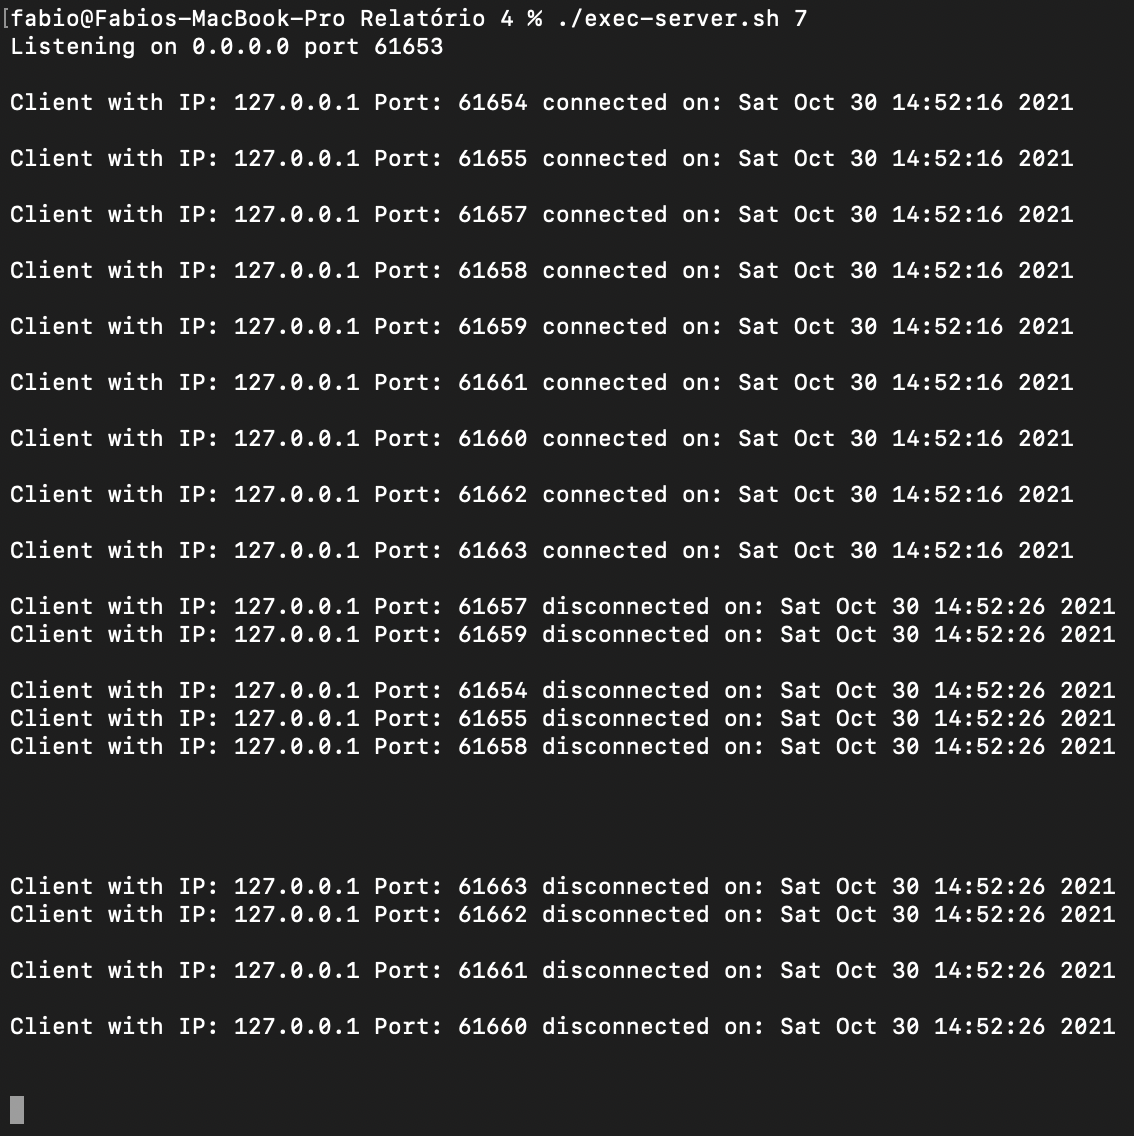
\includegraphics[width=1\textwidth]{images/servidor-backlog-7.png}
        Cliente:\\\\
        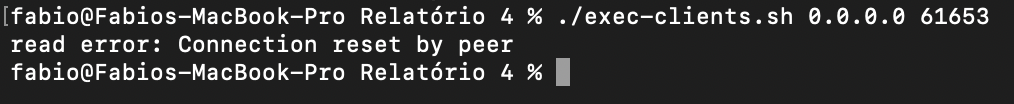
\includegraphics[width=1\textwidth]{images/cliente-backlog-7.png}
        Monitoramento:\\\\
        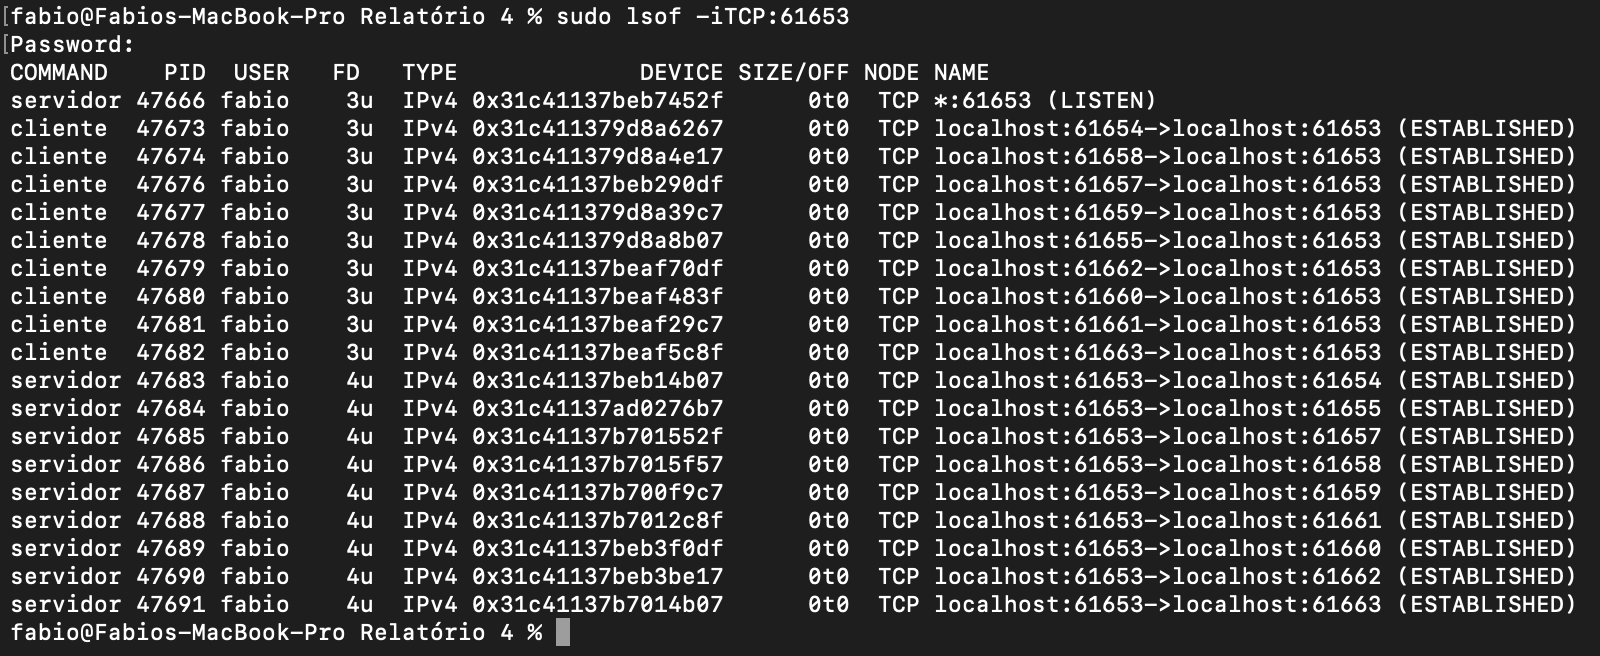
\includegraphics[width=1\textwidth]{images/lsof-backlog-7.png}
        
        \item Backlog = 8\\
        Servidor:\\\\
        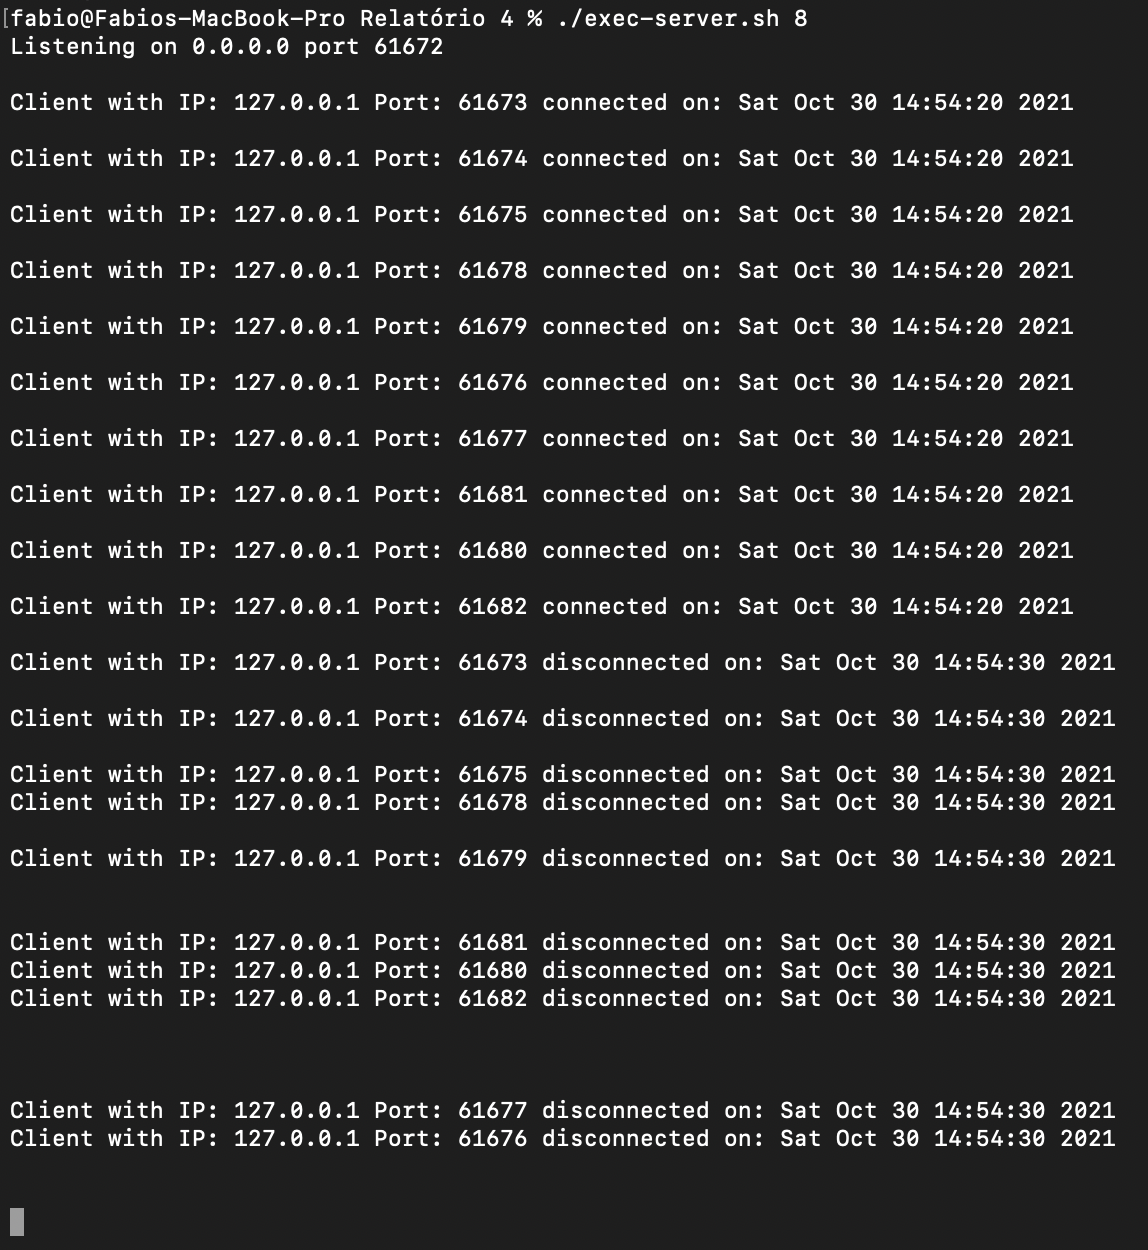
\includegraphics[width=1\textwidth]{images/servidor-backlog-8.png}
        Cliente:\\\\
        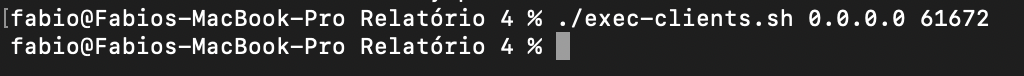
\includegraphics[width=1\textwidth]{images/cliente-backlog-8.png}
        Monitoramento:\\\\
        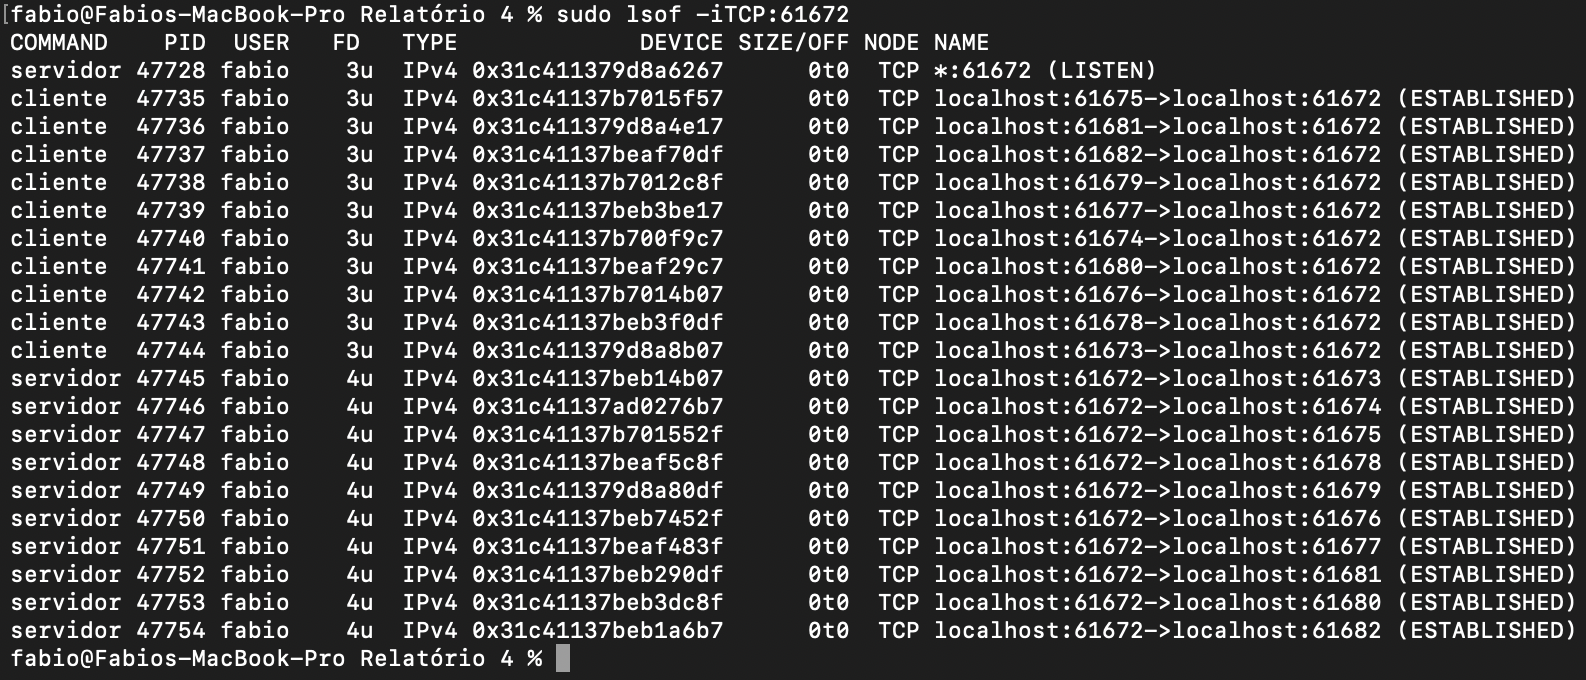
\includegraphics[width=1\textwidth]{images/lsof-backlog-8.png}
        
        \item Backlog = 9\\
        Servidor:\\\\
        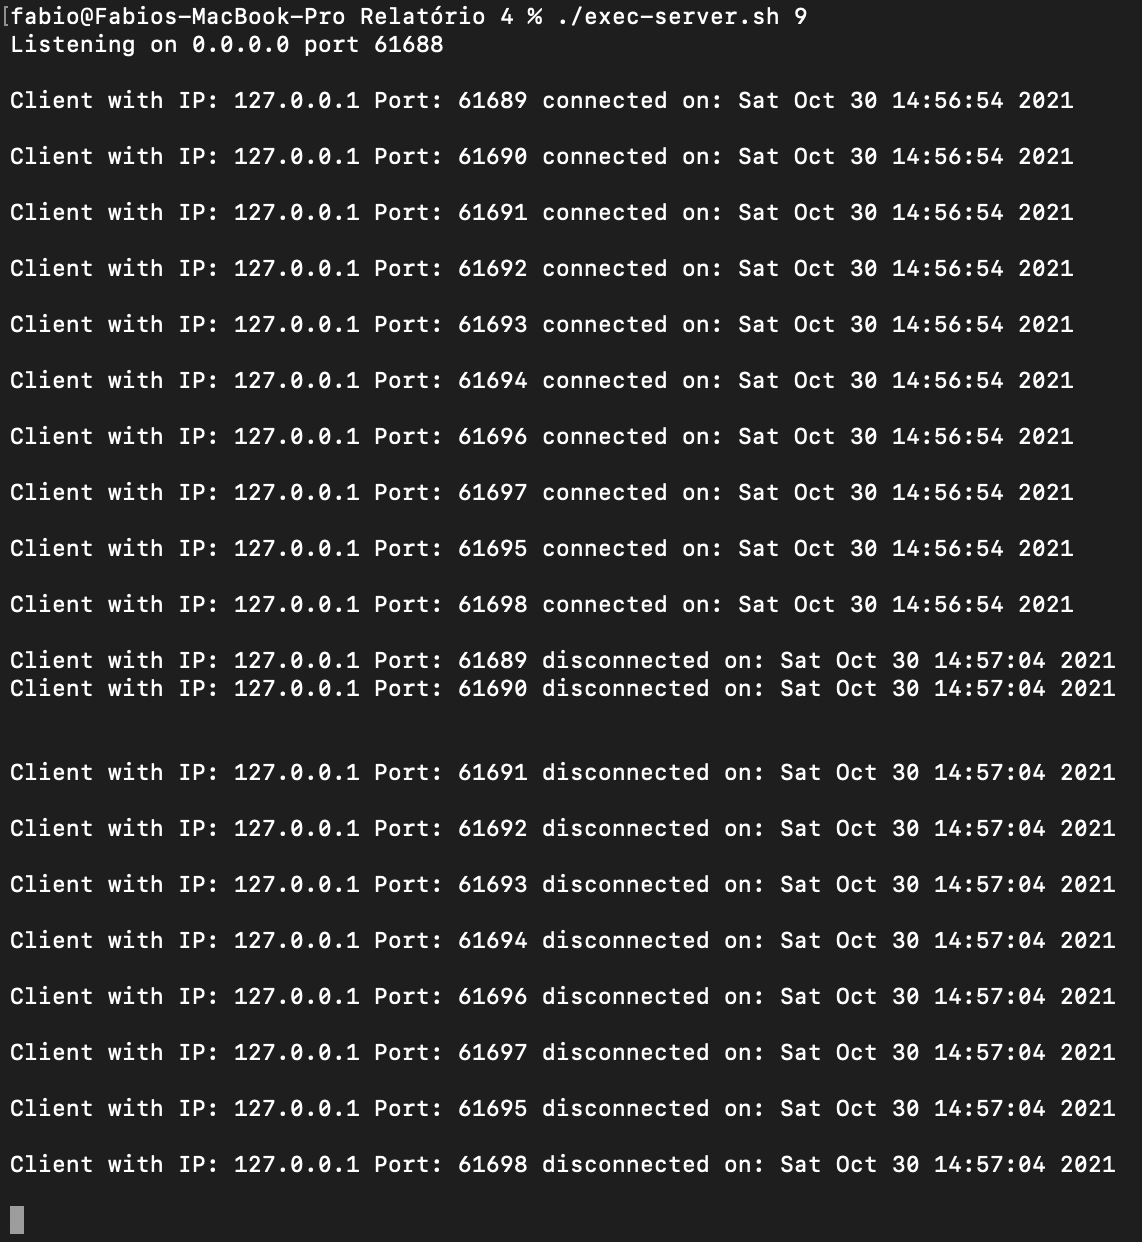
\includegraphics[width=1\textwidth]{images/servidor-backlog-9.png}
        Cliente:\\\\
        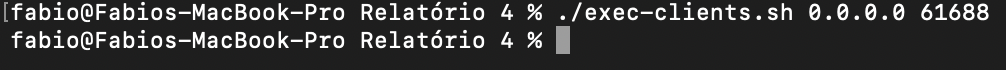
\includegraphics[width=1\textwidth]{images/cliente-backlog-9.png}
        Monitoramento:\\\\
        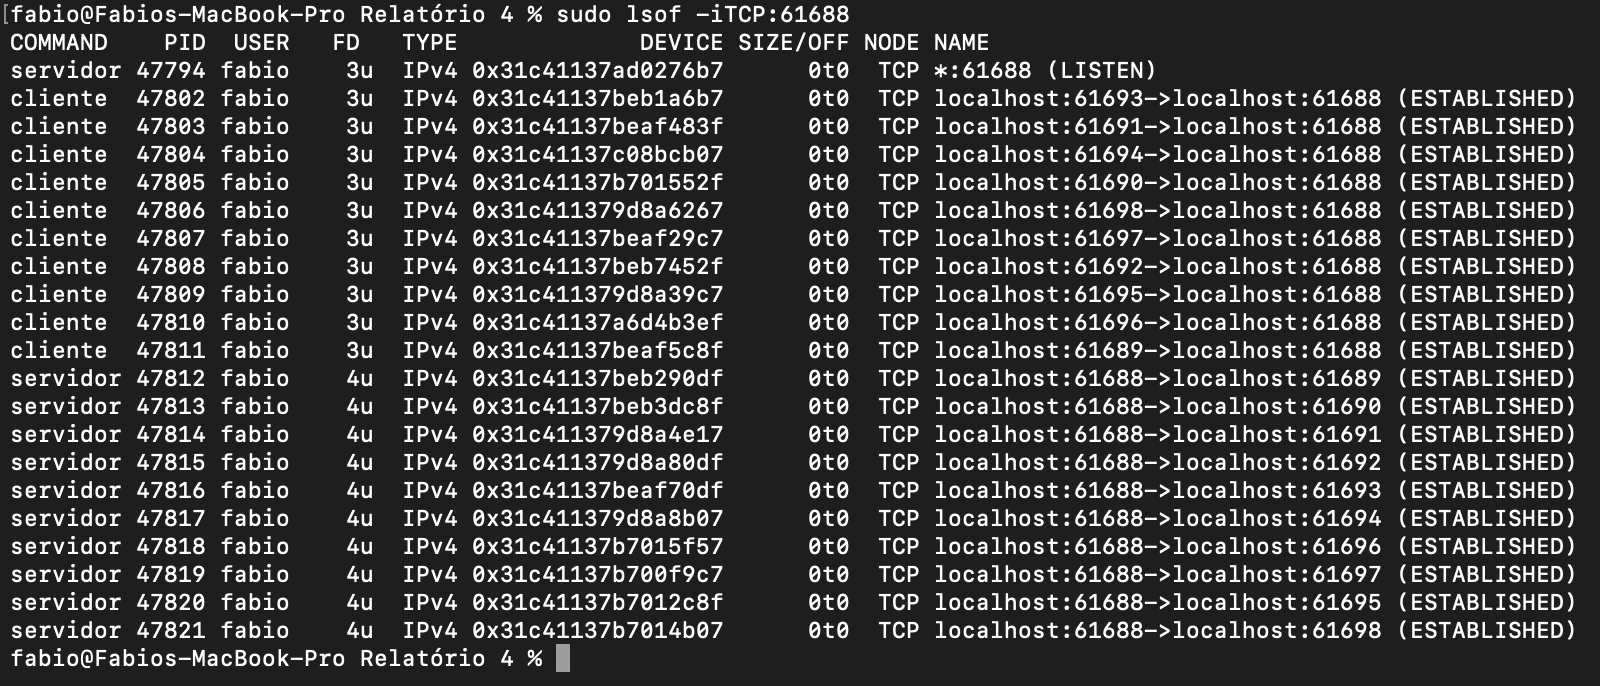
\includegraphics[width=1\textwidth]{images/lsof-backlog-9.png}
        
        \item Backlog = 10\\
        Servidor:\\\\
        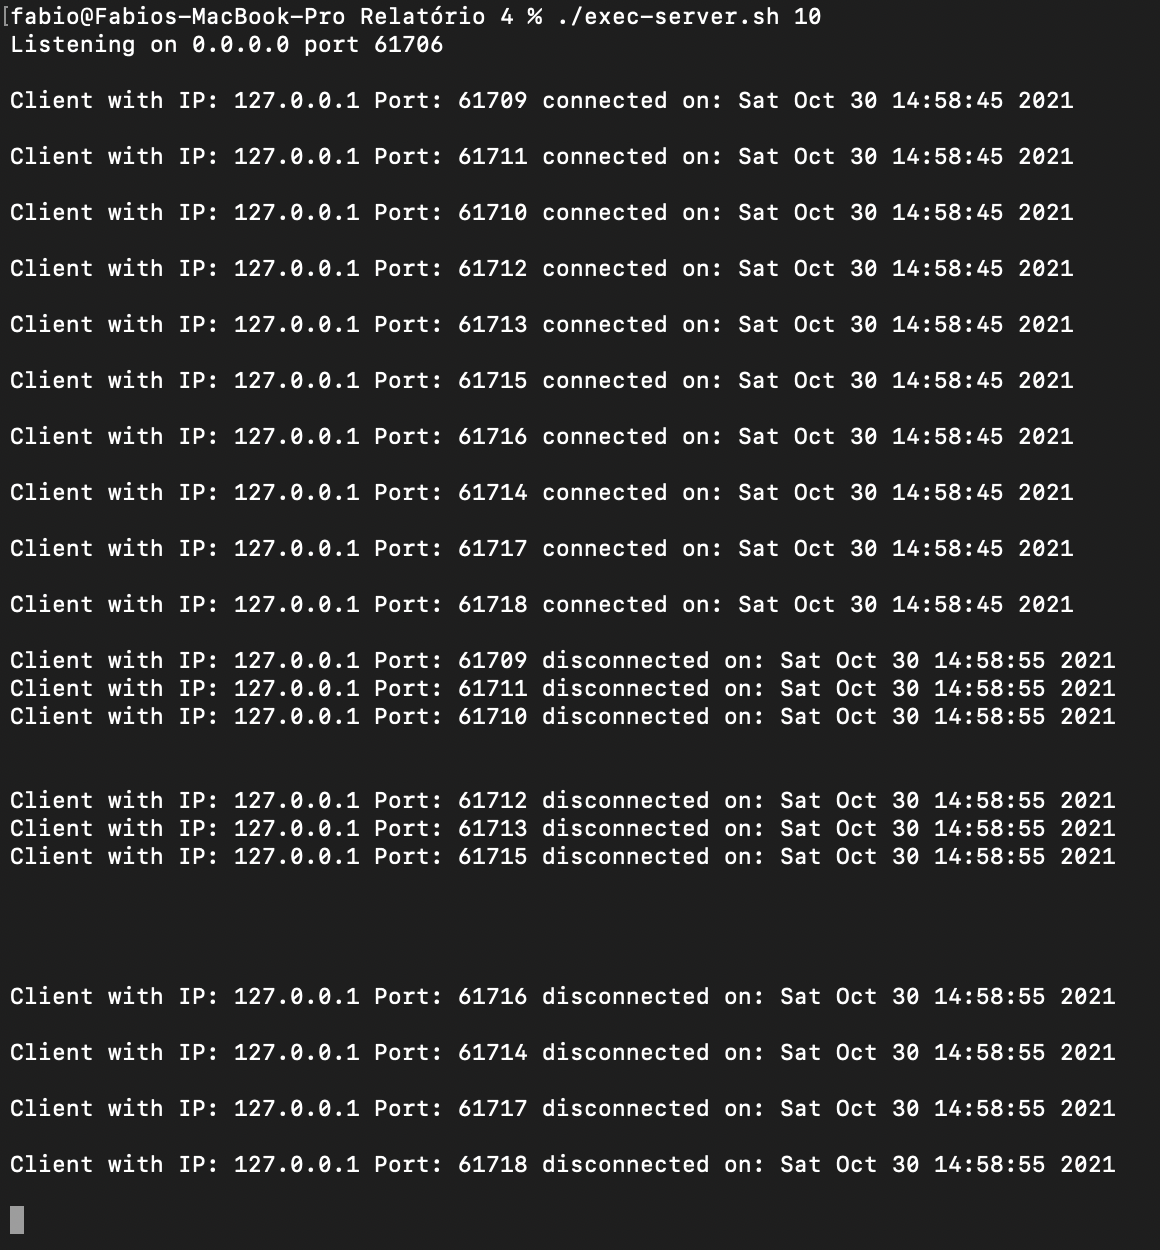
\includegraphics[width=1\textwidth]{images/servidor-backlog-10.png}
        Cliente:\\\\
        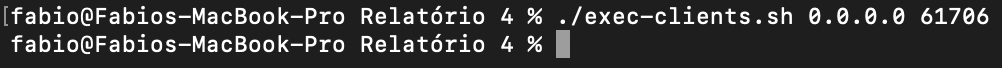
\includegraphics[width=1\textwidth]{images/cliente-backlog-10.png}
        Monitoramento:\\\\
        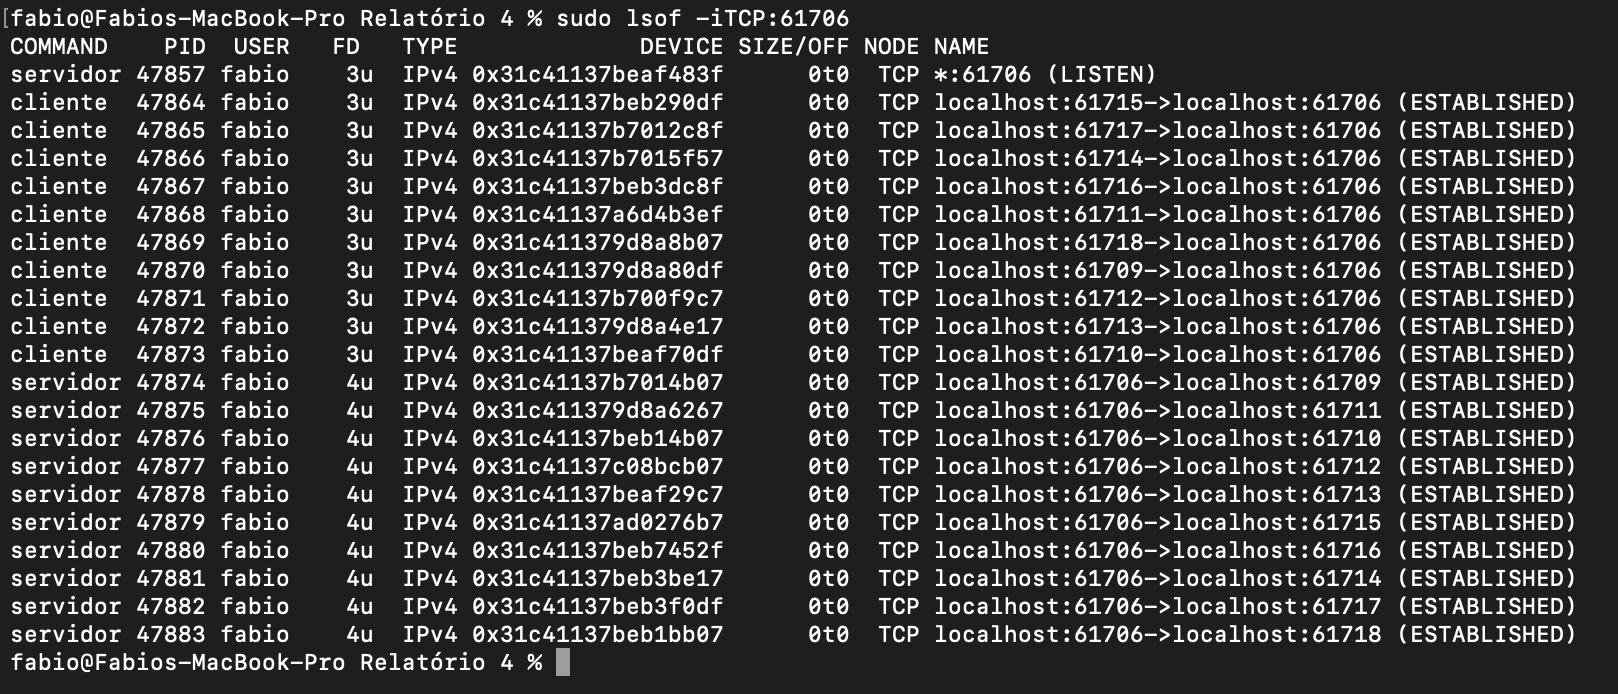
\includegraphics[width=1\textwidth]{images/lsof-backlog-10.png}
    \end{enumerate}
    
    Como esperado, nota-se que conforme aumenta-se o backlog, o número de clientes conectados com sucesso (estado \textbf{ESTABLISHED}) também aumenta. É possível ver também que quando um cliente não consegue realizar o 3 way hadshake do TCP com sucesso, imprime um "read error: Connection reset by peer", significando que o servidor desconsiderou essa conexão (não realizou o 3WHS).
    
    \item Não, o código atual não gera processo zumbi. Para constatar isso, executou-se um servidor, um cliente e monitorou-se a rede antes, durante e depois do cliente se desconectar.
    \\
    Servidor:\\\\
    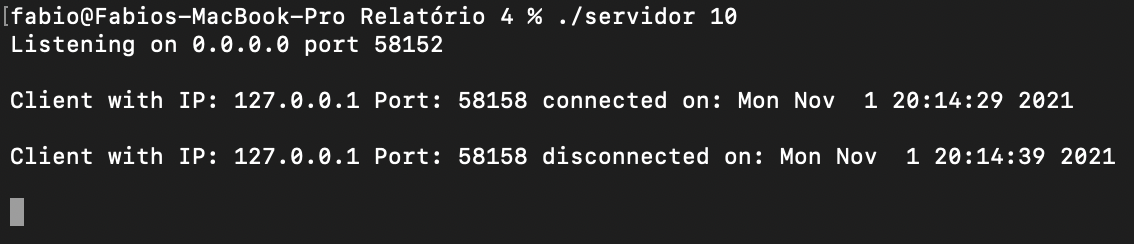
\includegraphics[width=1\textwidth]{images/ex5-servidor.png}
    Cliente:\\\\
    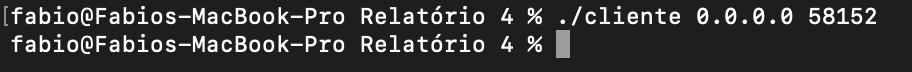
\includegraphics[width=1\textwidth]{images/ex5-cliente.png}
    Monitoramento:\\\\
    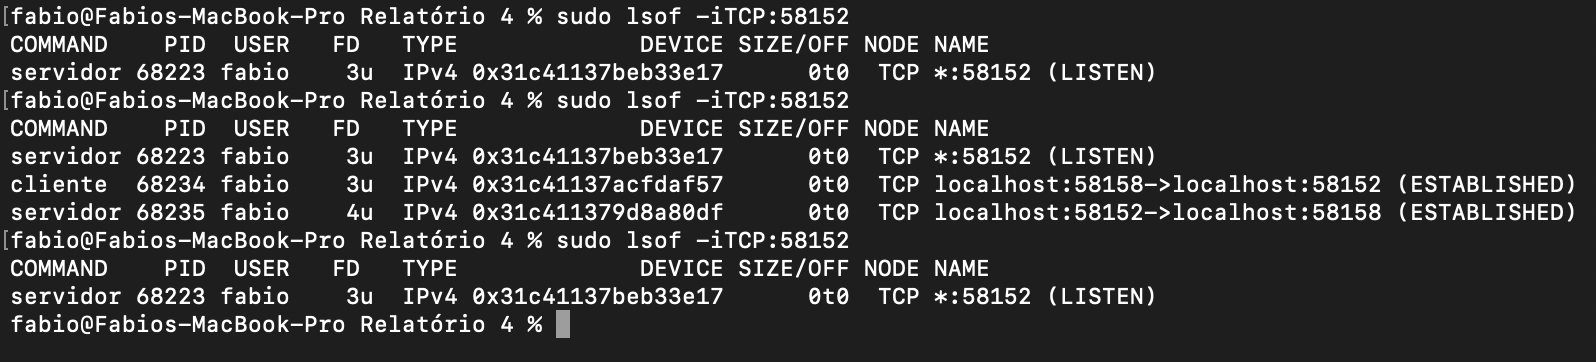
\includegraphics[width=1\textwidth]{images/ex5-lsof.png}
    Nota-se que antes da execução do cliente, há apenas o processo principal do servidor ativo, rodando no estado de LISTEN. Após a conexão de um cliente, são iniciados mais 2 processos, um no lado cliente e um processo filho do servidor, que tratará a conxexão em questão (ambos em estado ESTABLISHED). Finalmente, após a finalização da troca de mensagens, ambos os processos criados com a execução do cliente são finalizados, não aparecendo no monitoramento da rede.
\end{enumerate}

\end{document}
